\chapter{Spin Glass}
\label{chap:SGintro}
\section{Introduction and Experimental Features}
\label{sec:sg_intro}
Spin glasses \cite{Binder-Young-1986} are magnetic systems where the frozen-in quenched  
disorder leads to conflicting couplings among magnetic moments, which prevents the formation 
of long-range magnetic ordering, e.g.,ferromagnetic ordering.

The prototype material is a dilute magnetic alloy, with a small amount of 
magnetic impurity (such as Fe, Mn) randomly substituted into the lattice of a 
noble metallic host (i.e. Cu, Au). On the other hand, insulators such as 
Eu$_x$Sr$_{1-x}$S, and LiHo$_{x}$Y$_{1-x}$F$_{4}$ also show spin glass behavior.
 
The physics underlying the spin glass behavior comes from the quenched 
randomness: a pair of spins has a roughly equal a priori probability of having
a ferromagnetic or an anti-ferromagnetic interaction. For the dilute magnetic 
alloy, the conduction electron-mediated 
Ruderman-Kittel-Kasuya-Yosida (RKKY) interactions between the localized moments
 oscillates strongly with distance, 
 \begin{equation}
   \label{eq:RKKY}
   J(R)=J_0\frac{\cos(2k_FR+\phi_0)}{(k_FR)^3}, R\rightarrow 0
 \end{equation}
Here $J_0$ and $\phi_0$ are constants, and $k_F$ is the Fermi wave number of the
host metal. Since the distance between any pair of spins is random, some of the $R$
will be positive, some will be negative,
thus forming ferromagnetic/antiferromagnetic bonds randomly, and no spin 
alignment would satisfactory all exchange bonds. In the other words, the 
ground state energy cannot be obtained by minimizing the local energy 
of every pair of spins.

\begin{figure}[!h]
  \label{fig:rkky}
  \centering
  \includegraphics[width=0.5\textwidth]{img/RKKY.png}
  \caption{Sketch of RKKY interaction.}
\end{figure}

Experiments demonstrated many unusual features of spin glass materials.

\subsection{AC susceptibility}
The experimental observation of a sharp cusp in the AC susceptibility, first
carried out on a metallic AuFe by \citet{PhysRevB.6.4220}, as shown in as shown in Fig.\ref{fig:au-fe-cusp}, 
sparked the research on spin glass materials. 
%Similar cusps in low-field AC susceptibility also occur in other diluted 
%magnetic alloys such as CuMn, AgMn, AuMn, and AuCr.
\citet{THOLENCE1977875,:/content/aip/proceeding/aipcp/10.1063/1.30603,
:/content/aip/proceeding/aipcp/10.1063/1.30565} also found similar cusp occurring in PtMn alloys.
Upon applying a magnetic field, Cannella and Mydosh also found that even a weak
magnetic field strongly rounds the cusp of $\chi(T)$.

The AC susceptibility of spin glass also features pronounced frequency dependence. 
In figure \ref{fig:ac-chi-freq}, we show the AC susceptibility of CuMn for various
AC frequencies $\nu$ ranging from 10 Hz to 10,000 Hz. As shown in the figure, the
peak of $\chi(T)$ gradually shift to lower temperature with decreased $\nu$.
This is natural considering that as one probes the spin motion at longer time scales,
the slowing down and freezing of the spins tend to occur at lower temperatures.

\begin{figure}
  \centering
  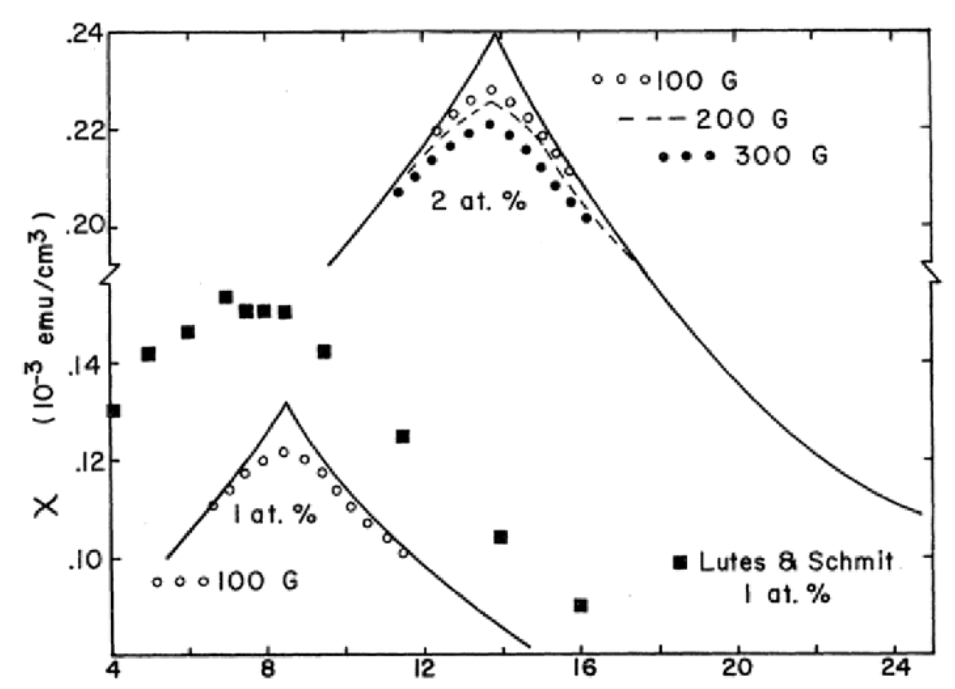
\includegraphics[width=0.6\textwidth]{img/cusp.png}
  \caption{\label{fig:au-fe-cusp}Susceptibility of Au-Fe alloys ploted vs. temperature. Full curves refer to zero field, from \citet{PhysRevB.6.4220}.}
\end{figure}
\begin{figure}
  \centering
  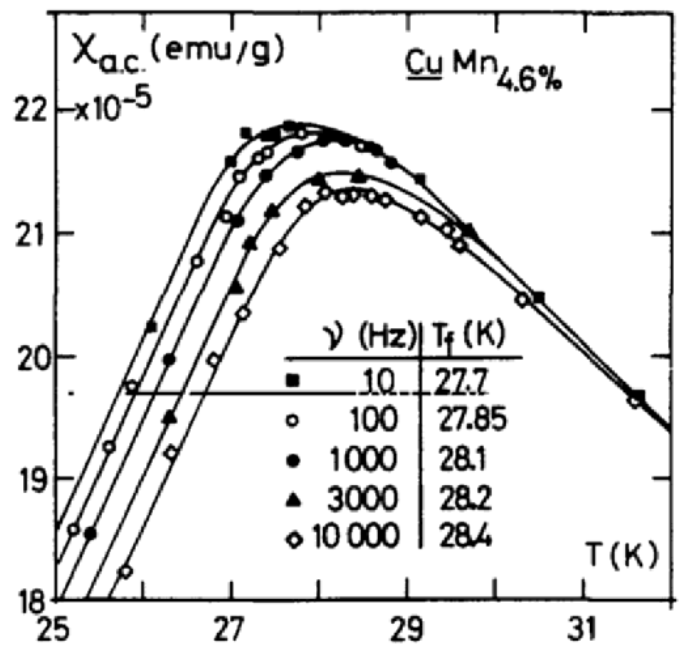
\includegraphics[width=0.5\textwidth]{img/ac-chi-freq.png}
  \caption{\label{fig:ac-chi-freq}The AC susceptibility of CuMn with 4.6\% Mn plotted vs temperature, for various ac frequencies, from \citet{THOLENCE1980113}.}
\end{figure}

%The cusp in the low-frequency AC susceptibility set off the theoretical interest of spin glass physics. 
These behaviors are in sharp contrast to conventional magnetic systems say a ferromagnet. 
The susceptibility diverges at the critical point, the susceptibility,
in this case, is the linear response function to the field. This can be understood 
as the conjugate variable of the magnetization, defined as 
$M=\lim_{N \rightarrow \infty} \langle s_{i}\rangle / N$, 
is the linear magnetic field. 
The spins point to a fixed preferential direction in the ordered phase. 
The cusp in the susceptibility has long been associated as the defining nature 
of a spin glass system. However, if the spin glass transition is a truly 
thermodynamic transition, we expect divergence in the response function
corresponding to the order parameter. 

It was soon found by Edwards and Anderson that the order parameter should be 
characterizing an order in which each individual spin can point to a fixed 
direction, but the direction of each spin is random. The original form of the 
Edwards-Anderson order parameter can be defined as 
$Q=\lim_{N \rightarrow \infty} \langle s_{i}\rangle^{2} / N$. 
It is clear the absence 
of the divergence in the usual linear response is due to that the conjugate 
variable of an external field does not diverge. If the magnetization is expanded 
in term of the magnetic field for two lowest orders, we can define
the nonlinear susceptibility, $M=\chi h - \chi_{nl} h^{3}$, where $\chi_{nl}$ is 
the nonlinear susceptibility. 
One can easily show that the nonlinear susceptibility is proportional to the 
spin glass susceptibility as the fluctuations of the Edwards-Anderson order 
parameter $Q$. 

The direct evidence of a thermodynamic spin glass transition can be deduced from 
the study of the non-linear susceptibility. The measurement is usually done by 
superconducting-quantum-interference-device (SQUID). The non-linear susceptibility 
can be extracted from the curve of the magnetization as a function of magnetic field.
This provides a direct access to the critical temperature and the exponent for the 
spin glass susceptibility. 


\subsection{Remanent Magnetization}
The magnetization process of spin glass is characterized by strong remanence effects.
Figure \ref{fig:trm-irm} shows remanent magnetization of AuMn measured in two ways:
the thermoremanent magnetization is measured by cooling the sample in a field $H$ 
from above $T_g$ to $T<T_g$, and removing the field afterward; the isothermal 
remanent magnetization is measured by first cooling down the sample in zero field to
below $T_g$, then applying a field and removing it. At lower fields, there is a 
clear difference between the two cases. Upon increasing $H$, the TRM increases to 
a maximum and the decrease, while the IRM shows a monotonic increase. With a large
magnetic field, both TRM and IRM saturate and agree. 


A particularly interesting feature of this irreversible behavior in spin glasses 
is the slow decay of the various remanent magnetizations with time. 
Relaxation phenomena occur below Tc on a typical timescale of 1 sec -- 1hr
\cite{tholence:jpa-00215633,Holtzberg1977,NIEUWENHUYS1977880}. This relaxation is distinctly non-exponential. It can be 
described in terms of power-laws\cite{NIEUWENHUYS1977880} or even, at not too late stages, by a 
logarithmic behavior\cite{Holtzberg1977} (see figure \ref{fig:au-fe-remanent}).

%including the cusp instead of a true divergence in the low-field, low-frequency 
%susceptibility and the discrepancy of magnetic response between zero-field and field cooling 
%measurements, as shown in Fig \ref{fig:experimentsSG}. 

\begin{figure}
  \centering
  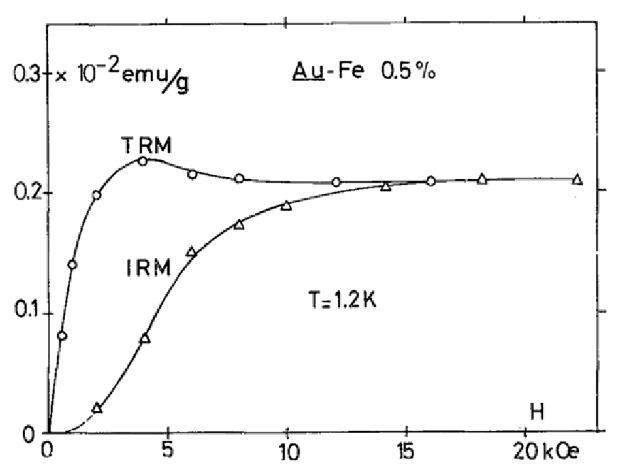
\includegraphics[width=0.6\textwidth]{img/trm-irm.png}
  \caption{\label{fig:trm-irm}The isothermal remanent magnetization (IRM) and 
thermoremanent magnetization (TRM) of AuMn with 0.5\% Mn vs magnetic field, 
from \citet{tholence:jpa-00215633}.}
\end{figure}

\begin{figure}
  \centering
  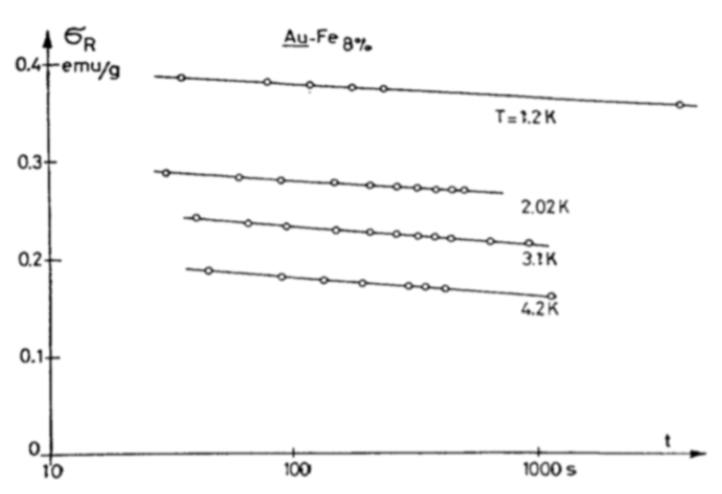
\includegraphics[width=0.6\textwidth]{img/remenant.png}
  \caption{ \label{fig:au-fe-remanent}Remanent magnetization of Au-Fe alloys plotted vs. time (logarithmic scale) for several temperatures, from \citet{Holtzberg1977}.}
\end{figure}
%Specific heat

\subsection{Specific Heat}

The specific heat of various spin glass materials has been measured and analyzed. 
In figure \ref{fig:cu-mn-cv}, we show the temperature dependence of magnetic 
specific heat of CuMn with 1.2\% Mn. The arrow on the x-axis indicates the spin glass
transition temperature $T_g$. The data shows a broad maximum above $T_g$, with no
anomaly at $T_g$. Below $T_g$, the specific heat exhibits $T$-linear behavior.

\begin{figure}
  \centering
  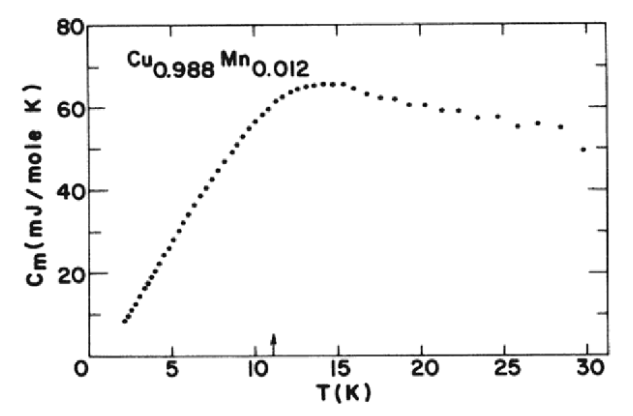
\includegraphics[width=0.6\textwidth]{img/cv.png}
\caption{\label{fig:cu-mn-cv}Magnetic part of specific heat of a Cu-Mn alloy plotted vs. temperature. Arrow shows where susceptibility has its cusp, from \citet{PhysRevB.13.4053}.}
\end{figure}

  

\iffalse
\begin{figure}[!h]
  \label{fig:experimentsSG}
  \centering
  \subfigure[Low frequency susceptibility of CuMn with 1\% Mn, from \citet{PhysRevB.23.1384}]
  {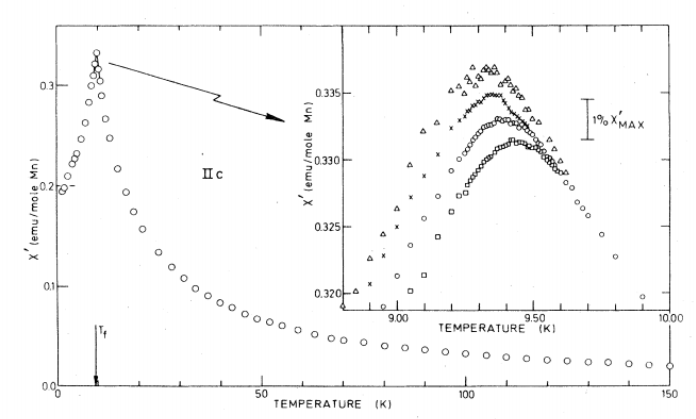
\includegraphics[width=0.6\textwidth]{img/cusp_low_freq.png}}\\  
\subfigure[Susceptibilities of CuMn vs temperature for 1.08\% and 2.02\% Mn, from 
\citet{PhysRevB.19.1633}]
{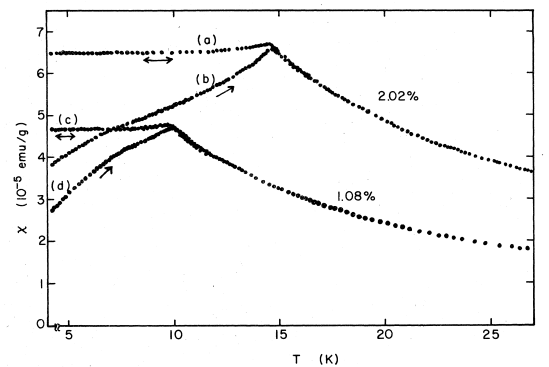
\includegraphics[width=0.6\textwidth]{img/fc_zfc.png}}
  \caption{Magnetic features of spin glass in a small field.}
\end{figure}
\fi


Other properties, such as DC susceptibility\citep{PhysRevB.19.1633,doi:10.1143/JPSJ.62.4488}, 
imaginary part of AC susceptibility\citep{PhysRevB.25.515,:/content/aip/journal/jap/53/3/10.1063/1.330780}, etc.,
were also extensively studied. 
These experimental facts suggest that spin glass system has no conventional 
long range magnetic ordering and exhibits very slow dynamics. For experimental 
systems, equilibrium can never be achieved. 



\section{Theoretical Understanding on Spin Glass}
A simple model that captures the consequences of disorder is an Ising model 
with quenched randomly disordered couplings, first proposed by Edwards and 
Anderson\cite{Edwards-Anderson1975}:
\begin{equation}
  \label{eq:Edwards-Anderson}
  H=-\sum_{\langle i,j \rangle}J_{ij}S_iS_j-h\sum_iS_i
\end{equation}
Here $S_i$ is the spin in a $d$-dimensional lattice that can take values $\pm 1$,
$\langle i,j \rangle$ indicates nearest neighbors with the coupling $J_{ij}$ between 
them, and $h$ is the external field.
 
Numerical evidence suggests that the criticality of the three-dimensional
spin glass systems are largely independent of the distribution of the randomness,
that is they are in the same universality class for different distributions. 
But, the two main paradigmatic cases for the $J_{ij}$ in Edwards-Anderson model are:
\begin{itemize}
\item Gaussian distribution of random coupling:
  \begin{equation}
    \label{eq:Jij_Gaussian}
    P(J_{ij})=\frac{1}{\sqrt{2\pi}}\exp^{-J_{ij}^2/2}
  \end{equation}
\item Bimodal ($\pm J$) distribution of random coupling:
  \begin{equation}
    \label{eq:Jij_bimodal}
    P(J_{ij})=\frac{1}{2}[\delta(J_{ij}-1)+\delta(J_{ij}+1)]
  \end{equation}
\end{itemize}

\subsection{Frustration}
\label{sec:frustration}
Frustration naturally presents in the Hamiltonian in Eq \ref{eq:Edwards-Anderson}, when no spin 
configurations can satisfy all couplings at the same time. 
Figure \ref{fig:frustration} demonstrate two situations where frustrations 
happens. In Fig \ref{fig:frustration_geo}, the two spins on the top and the left
are anti-parallelly aligned due to the antiferromagnetic coupling between them,
but there is not a preferred spin direction for the third spin that can satisfy
both the antiferromagnetic bonds. In Fig \ref{fig:frustration_quench}, the 
frustration comes from the random distribution of $J_{ij}$. 

\begin{figure}
  \centering
  \subfigure[Geometrical Frustration. Here all couplings are anti-ferromagnetic.]{
    \label{fig:frustration_geo}
    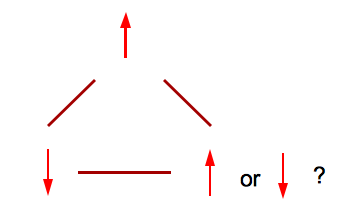
\includegraphics[width=0.4\textwidth]{img/ising-3-spin.png}
  }\hspace{0.5cm}
  \subfigure[Frustration due to randomness. Here $J=-1$ indicates an 
anti-ferromagnetic coupling, while $J=+1$ means ferromagnetic coupling.]{
    \label{fig:frustration_quench}
    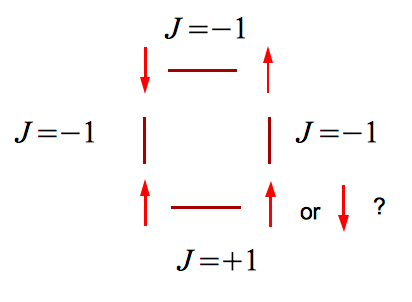
\includegraphics[width=0.4\textwidth]{img/ea-4-spin.png}
  }
  \caption{Frustration in Edwards-Anderson model.}
  \label{fig:frustration}
\end{figure}

The frustration is a key factor that leads to many features which make 
spin glass a complex system.
These features include: the existence of many metastable states; the rugged energy 
landscape; and dynamical behaviors such as slow relaxation, irreversibility, 
memory effects, hysteresis, etc. 


\subsection{Pictures on the Nature of the Spin Glass Phase}
\label{sec:meanfield-model}

An infinite-ranged version of spin glass models 
was proposed by Sherrington and Kirkpatrick (SK) \cite{Sherrington-Kirkpatrick-1975,Sherrington-Kirkpatrick1978}.
\begin{equation}
  \label{eq:SK}
  H=-\frac{1}{\sqrt{N}}\sum_{1\le i\le j\le N}J_{ij}S_iS_j
\end{equation}
Here $J_{ij}$ is chosen from a Gaussian distribution in equation 
\ref{eq:Jij_Gaussian}.
This model has an equilibrium phase transition at $T_c = 1$.
For the spin glass phase below $T_c$, Parisi\cite{Parisi1980,Parisi-1980b,Parisi-1980a} employed a novel ansatz and 
developed a  possible physical interpretation of the nature of spin glass, 
which is now known as the ``Replica Symmetry Breaking'' (RSB) picture. The main
idea behind the picture is that the spin glass phase consists of an infinite 
number of ``pure states'' that form a hierarchy rather than follow simple symmetry
transformation. 
The ultrametric topology of spin glass states can be represented with a 
genealogical tree. Each end point corresponds to a pure state, and branches 
represent clusters, as sketched in Fig. \ref{fig:TreeRSB}. 

%http://lptms.u-psud.fr/membres/Mezard/Pdf/84_MGSTV_PRL.pdf
%insert tree picture here.

\begin{figure}[!h]
  \label{fig:TreeRSB}
  \centering
  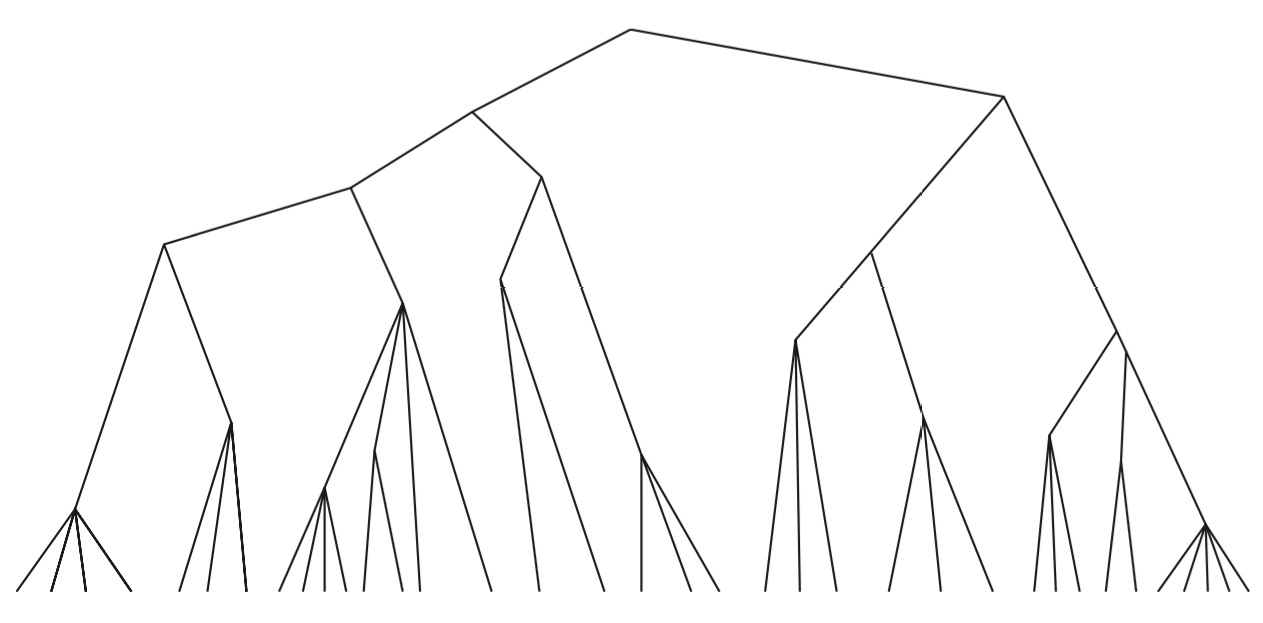
\includegraphics[width=0.6\textwidth]{img/TreeRSB.png}
  \caption{Hierarchical structure of the ensemble of spin-glass states, according
to the replica symmetry breaking picture. The end points represents states; branches (with all their descendents)
represent clusters.}
\end{figure}


Replica symmetry breaking is successful in the description of infinite range models, but whether it 
holds in finite dimensions remains the most prominent open question in the study of spin glass systems. 
A competing picture, known as droplet/scaling\cite{Fisher-Huse-1987,Fisher-Huse-1988}, 
is based on domain-wall 
renormalization group ideas. In this picture, there is only a single of
pure states that are spin-flip-symmetrical at low temperature in any finite 
dimension. The difference between the consequence from these two pictures 
will show up in the order parameters for spin glass as we will define in the following.

%\section{Quantities characterizing spin glass}

The quantity $q$ measures the overlap of the samples after a long time relaxation process. 
It was first studied by the seminal paper by Edwards and Anderson,
\begin{equation}
  \label{eq:q}
  q=\frac{1}{N}\sum_iS_i^\alpha S_i^\beta=\frac{1}{N}\lim_{T\to \infty}\sum_iS_i(t_0)S_i(t_0+T)
\end{equation}
where $\alpha$ and $\beta$ are two copies of lattice with the same disorder 
configuration, but simulated with different random seeds, so they are
statistically independent of each other. The Edwards-Anderson order paremeter, q, 
is the order parameter of measuring the breaking of ergodicity. 

The order parameter defined for the spin glass measuring the change of the systems
when the time goes to infinity. In the thermodynamic limit, if this
is zero, the system is ergodic, if this is finite, the system breaks
the ergodicity. Some parts of the phase space can never be sampled.

In contrast to conventional order parameters which measures the 
spatial pattern, such as magnetization. If the order parameter is non-zero, 
the system is said to undergo spontaneous symmetry breaking, in which the symmetry of 
the states is lower than that of the Hamiltonian. If one calculates
the Edwards-Anderson order parameter, said for the ferromagnet, it will
show a finite value. However, this is not a spin glass transition, a
spin glass transition does not come with a spontaneous symmetry breaking in space.

According to the Parisi solution, for fixed J and (large) N, the structure of 
the overlap is nontrivial, while in droplet picture, in the thermodynamic limit, 
the distribution is just a pair of delta functions at $\pm 1$. 
%insert figure for RSB/droplet overlap here

\begin{figure}
  \centering 
  \subfigure[Replica symmetry breaking picture]{
    \label{fig:overlap_rsb}
    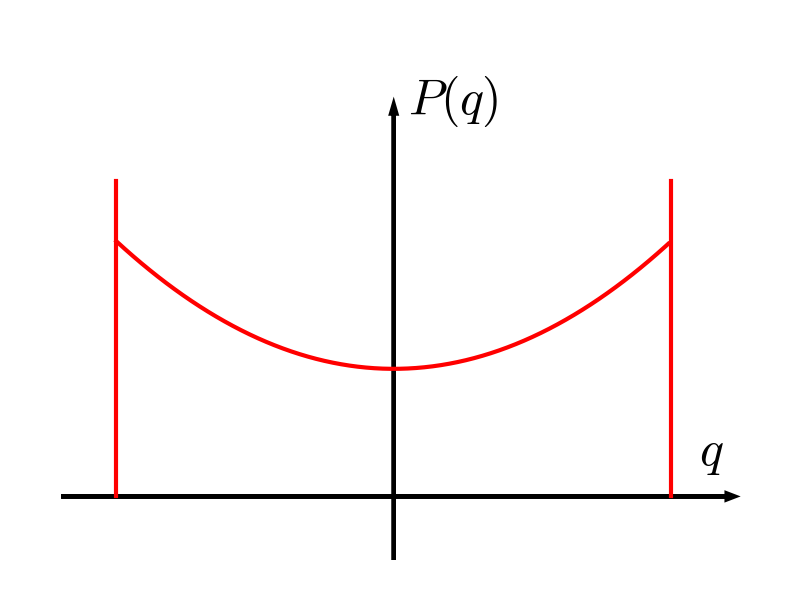
\includegraphics[width=0.4\textwidth]{img/sg/sg_rsb.png}
  }\hspace{0.5cm}
  \subfigure[Droplet picture]{
    \label{fig:overlap_droplet}
    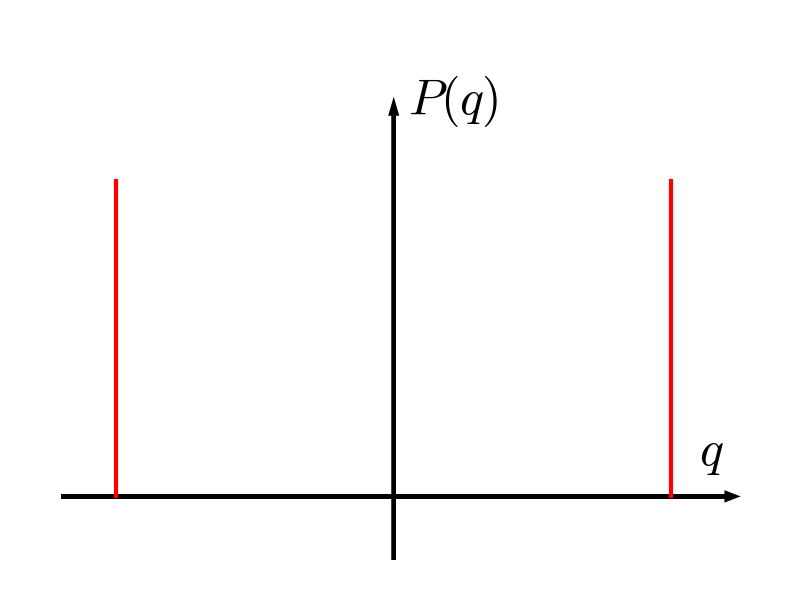
\includegraphics[width=0.4\textwidth]{img/sg/sg_droplet.png}
  }
  \caption{Sketch of the overlap distribution $P(q)$ for the replica symmetry 
breaking picture, and the droplet picture.}
  \label{fig:overlap}
\end{figure}

\section{Finite Size Scaling}
Most phase transitions can be described by an order parameter, which measures
the degree of order in a system. Usually, an order parameter is zero in one phase,
and non-zero in the other. At the critical point, the susceptibility of the order
parameter should diverge at the thermodynamic limit. An example of an order parameter is the 
magnetization in a ferromagnetic system. 
 
Second-order phase transitions, such as the magnetic transition in the Ising model, and 
spin glass transition in the Edwards-Anderson model, can be characterized by their 
power law behaviors for various quantities, such as heat capacity and susceptibility,  
close to the critical point. The systems can be categorized into different universality 
class according to the values of the exponents of these power law behaviors. For example, 
\begin{equation}
  \label{eq:20}
  \begin{array}{lrcl}
    \mathrm{Magnetization}& M& \sim& \left|T-T_c\right|^\beta\\
    \mathrm{Magnetic~susceptibility}& \chi_M& \sim& \left|T-T_c\right|^{-\gamma}\\
    \mathrm{Heat~capacity}& C_V& \sim& \left|T-T_c\right|^{-\alpha}\\
    \mathrm{Correlation~length}& \xi& \sim& \left|T-T_c\right|^{-\nu}
  \end{array}
\end{equation}

Close to the critical temperature, one can use the following ansatzes:
\begin{equation}
  \label{eq:17}
  M=L^{-\beta/\nu}g_M(tL^{1/\nu})
\end{equation}
\begin{equation}
  \label{eq:19}
  \chi=L^{\gamma/\nu}g_\chi(tL^{1/\nu})
\end{equation}
\begin{equation}
  \label{eq:18}
  C_V=L^{\alpha/\nu}g_C(tL^{1/\nu})
\end{equation}
where $t=(T-T_c)/T_c$.

A frequently used method to determine the critical point is to use
the intersection points of the Binder cumulants:
\begin{equation}
  \label{eq:14}
  U_L=\frac{1}{2}\left(3-\frac{\langle M^4\rangle_L}{\langle M^2\rangle^2_L}\right)
\end{equation}

For $T>T_c$, $\langle M^4\rangle_L = 3 \langle M^2\rangle_L^2$. 
For $T<T_c$, $\langle M^4\rangle_L = \langle M^2\rangle_L^2$.

As a result, the binder ratio
\begin{equation}
  \label{eq:16}
  U_L=\frac{1}{2}\left(3-\frac{\langle M^4\rangle_L}{\langle M^2\rangle^2_L}\right)
  =\left\{
    \begin{array}{ccc}
      0 & \mathrm{for} & T>T_c\\
      1 & \mathrm{for} & T<T_c
    \end{array}
  \right.
\end{equation}

At $T_c$, the Binder ratio does not depend on $L$ since
\begin{equation}
  \label{eq:15}
  \frac{\langle M^4\rangle_L}{\langle M^2\rangle^2_L}
  =\frac{L^{-4\beta/\nu}g_{M^4}(tL^{1/\nu})}{\left(L^{-2\beta/\nu}g_{M^2}(tL^{1/\nu})\right)^2}
  =g_c(tL^{1/\nu})
\end{equation}
therefore, $U_L$ tends towards an universal value independent of the system size.

So one can use various system sizes $L$, calculate $U_L$s as functions of $T$,
and find the point where the $U_L(T)$ curve cross to identify $T_c$. The catch
of the finite size scaling is that the power law scaling behavior is valid
only for the system is large, usually one would like to have the system
sizes to be larger than the correlation length. Even though, the finite size
scaling can in principle extract the exponent of the thermodynamic system,
it is still desirable to simulate large system sizes.
  
\section{Difficulties and Outstanding Problems}
The Edwards-Anderson model is a deceptively simple problem. Since it is a classical spin 
model, one may think that its numerical study can be simply carried out by Monte
Carlo methods on conventional hardware. One of the defining signatures of spin glass 
systems is their long relaxation time. 
For sufficiently low temperatures, the system becomes very sluggish and 
equilibration is prohibitively difficult even for modest systems sizes. 
Moreover, it has been shown that finding the ground state of the three-dimensional
Edwards-Anderson model is an NP-hard problem. \cite{Barahona-1982} 
Until recently, there has been no consensus on whether there is a finite spin 
glass critical temperature in the three-dimensional Edwards-Anderson model.

%It also requires a large number of disorder realizations to reach any 
%meaningful result.

Due to the difficulty in the simulation, there is still no general consensus on
which of the two competing pictures is correct. 
An import discriminator between the theories is the predicted behavior of 
the system when the temperature is decreased in the presence of an applied magnetic
field. 
In the mean-field approximation, the de Almeida-Thouless line separates the 
high-temperature paramagnetic phase from the spin glass phase (Fig.\ref{fig:at_rsb}). 
With the droplet/scaling theory, an applied magnetic field is predicted to remove
the phase transition completely (Fig.\ref{fig:at_droplet}).

\begin{figure}
  \centering
  \subfigure[Replica symmetry breaking picture]{
    \label{fig:at_rsb}
    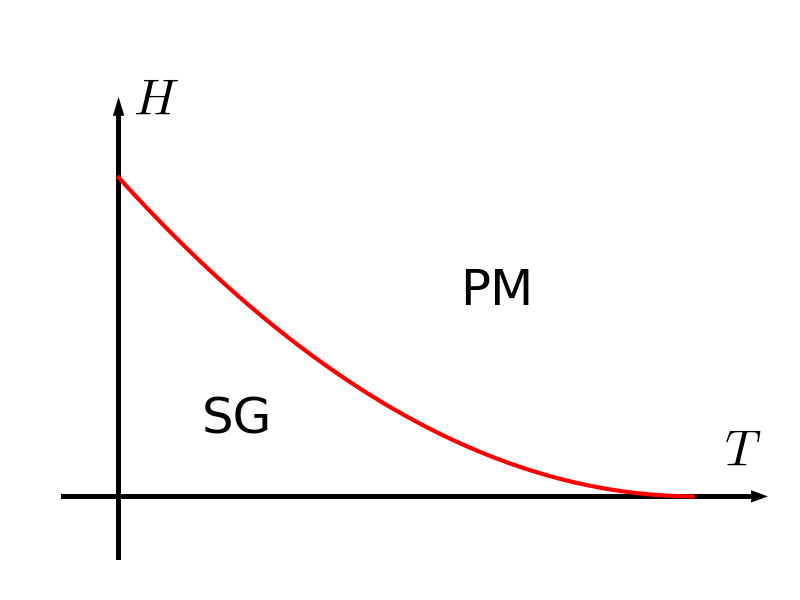
\includegraphics[width=0.4\textwidth]{img/sg/at_rsb.png}
  }\hspace{0.5cm}
  \subfigure[Droplet picture]{
    \label{fig:at_droplet}
    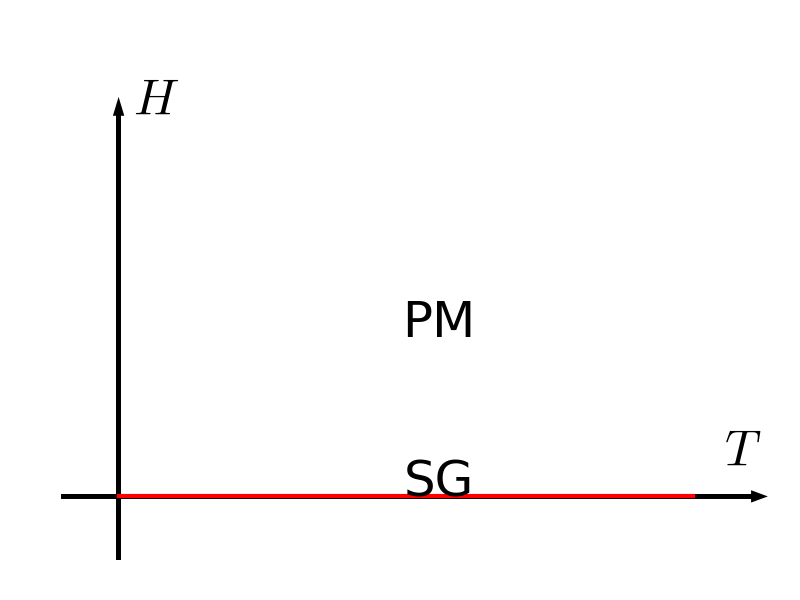
\includegraphics[width=0.4\textwidth]{img/sg/at_droplet.png}
  }
  \caption{Sketch of the de Almeida-Thouless line in the replica symmetry breaking 
picture, and the droplet picture.}
  \label{fig:at_line}
\end{figure}

Recent work supports that there is only a pair of two ground states in two dimensions.
In four dimensions, the JANUS show evidence for the presence of a spin glass
phase transition in a field. In three dimensions, numerical simulations give 
conflicting results.


\section{Algorithms for Spin Glass Simulation}
The breakthrough in the numerical study of spin glass systems came with the 
introduction of the parallel tempering method\cite{Swendsen-Wang-1986,Hukushima-Nemoto1996,Marinari-Parisi1992}. 
Parallel tempering (PT), also known
as replica exchange, is a simulation method aimed at improving the dynamic 
properties of Monte Carlo sampling. Instead of simulating one Markov chain at 
a time, one runs N copies of the system with random seeds at different 
temperatures and exchange configurations based on the detailed balance condition.
By making the configurations at high temperatures available to simulations at 
low temperatures, this method allows better sampling over the entire energy
landscape. We discuss this method further in \ref{sec:PT}.

Simulated annealing\citep{1983Sci...220..671K} is another commonly used algorithm for heuristic optimization,
due to its simplicity and effectiveness. In physics, one usually select the 
energy as the cost function, start the Monte Carlo simulation at a high temperature
and slowly tune down the temperature during the simulation, and in the end, the
configuration of the system would stay in a local minimum. With slow-enough annealing
and multiple repetitions, one would expect to find the global minimum.  

Population annealing\citep{2015PhRvE..92f3307W} combines simulated annealing and Boltzmann weighted 
differential reproduction within a population of replicas to sample equilibrium 
states. Similar to simulated annealing, population annealing involves lowering 
the temperature of the system at a sequence of temperatures. However, population annealing uses a 
population of replicas and this population is resampled at each time step.
By doing this, population annealing aims to ensure that the population always stay close to the 
Gibbs distribution. Population annealing is naturally a massively
parallel algorithm, as realistic spin glass simulation using population 
annealing require population sizes of the order $10^6$ or more.
%http://arxiv.org/pdf/1508.05647v2.pdf

Another possibility to overcome the diverging autocorrelation time problem is the 
multicanonical reweighting method\citep{1998PhyA..254..164J}. Instead of sampling the Boltzmann 
distribution $P=\exp(-\beta Ep)$, multicanonical ensemble uses the 
Metropolis–Hastings algorithm with a sampling distribution given by the inverse 
of the density of states of the system. The density of states has to be known 
a priori or be computed using techniques such as the Wang and Landau algorithm.



%%% Local Variables:
%%% mode: latex
%%% TeX-master: "../thesis"
%%% End:
